\chapter{Methodology}

In this chapter,
the methodological approach,
as well as
the used scientific research methods
are presented.


\section{Approach}

% TODO: add activity 1-6 to illustration?

To achieve the main goal of the thesis and answer the identified RQs,
a mix of different scientific methods will be used.
In order to help with the recognition and legitimization of the conducted research,
a commonly accepted framework, namely
the methodology for conducting design science (DS) research
in information systems (IS)
\autocite{designScienceResearchMethodologyForInformationSystemsResearch}
will be applied.
It consists of six activities
(illustrated in Figure \ref{fig:dsrmProcessReleasePromotionGitOps}):

\begin{itemize}
	\item \nameref{methodology:activity1}
	\item \nameref{methodology:activity2}
	\item \nameref{methodology:activity3}
	\item \nameref{methodology:activity4}
	\item \nameref{methodology:activity5}
	\item \nameref{methodology:activity6}
\end{itemize}

%Since the model allows for process iteration,
%it will be decided by the researcher
%whether, at the end of activity 5,
%to iterate back to activity 3 to try to improve the artifact.
The process is structured in a nominally sequential order.
For this concrete research,
the problem-centered initiation is chosen as the entry point,
thus the process will begin with activity 1.
Afterwards the research will proceed sequentially,
because the idea of the research resulted from observation of the problem
\autocite{designScienceResearchMethodologyForInformationSystemsResearch}.
\bigskip

\begin{figure}[h]
	\centering
	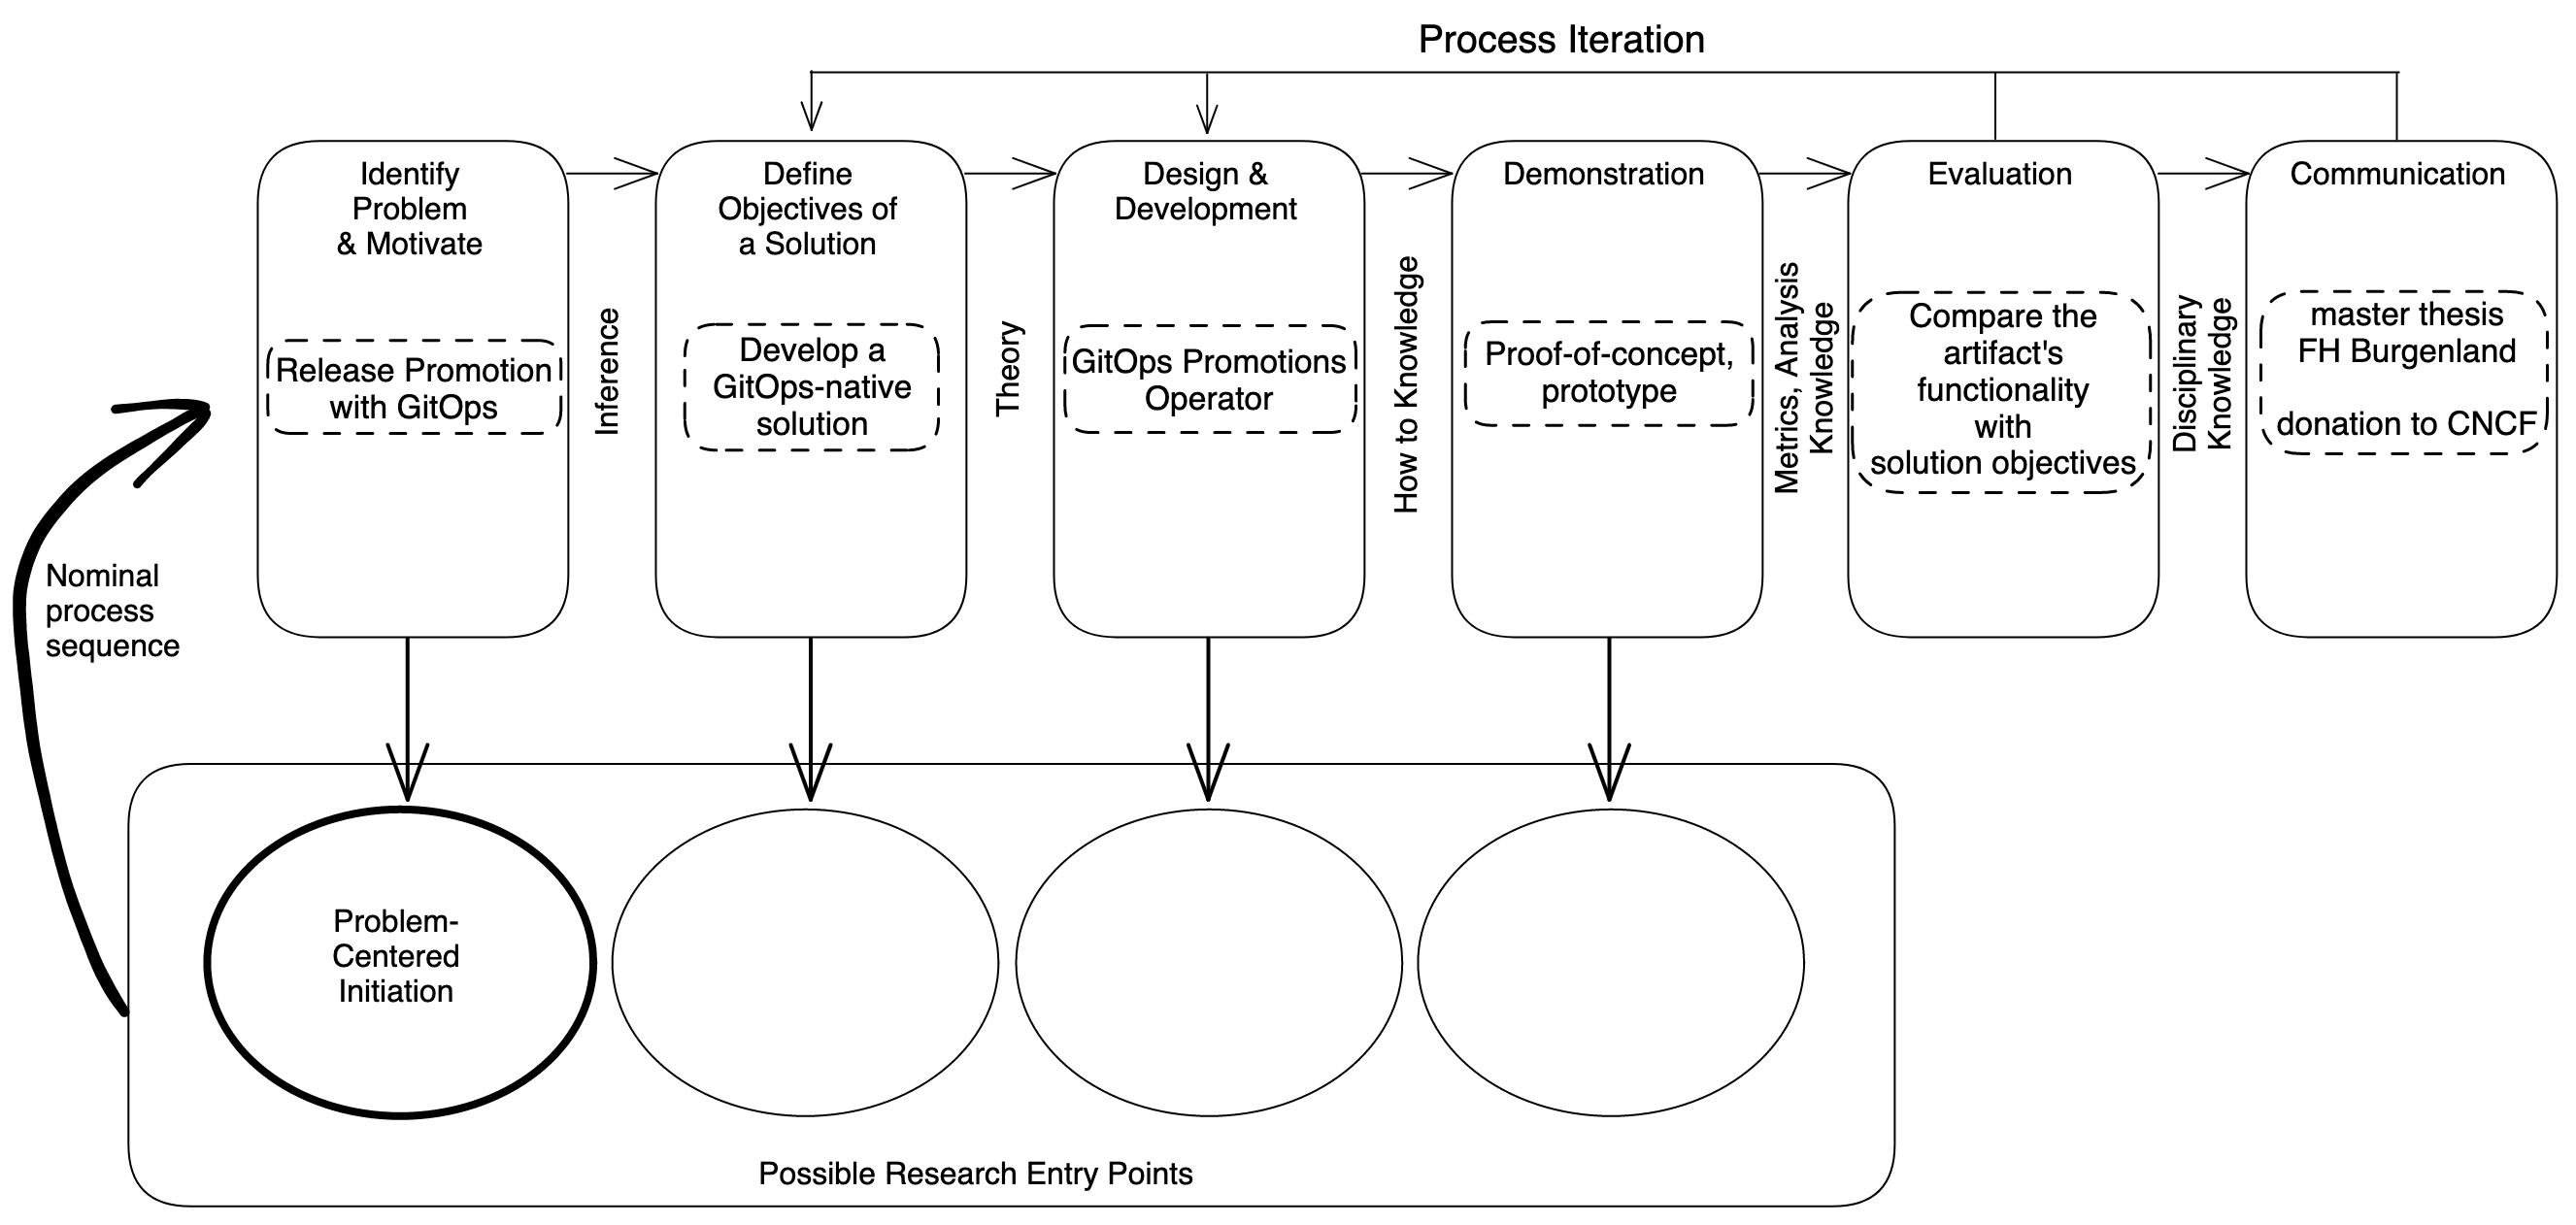
\includegraphics[width=1.00\linewidth]{figures/dsrm-process-release-promotion-gitops.png}
	\caption{DSRM Process for this thesis.
		%		(\citeauthor{ref}, \citeyear{ref}).
	}
	\label{fig:dsrmProcessReleasePromotionGitOps}	
\end{figure}

\subsection{Activity 1: Identify Problem \& Motivate}
\label{methodology:activity1}

\noindent
In activity 1,
the research problem of
release promotion with GitOps
is defined.
This is accomplished, by
seeking knowledge of the state of the problem
from practicing professionals,
as well as analysing prior written literature.
To assist later evaluation,
the problem is conceptually broken down into distinct items.
The value of a solution is highlighted,
in order to help the audience of the research
understand the reasoning associated with the
researcher's understanding of the problem
\autocite{designScienceResearchMethodologyForInformationSystemsResearch}.
\bigskip

\begin{figure}[h]
	\centering
	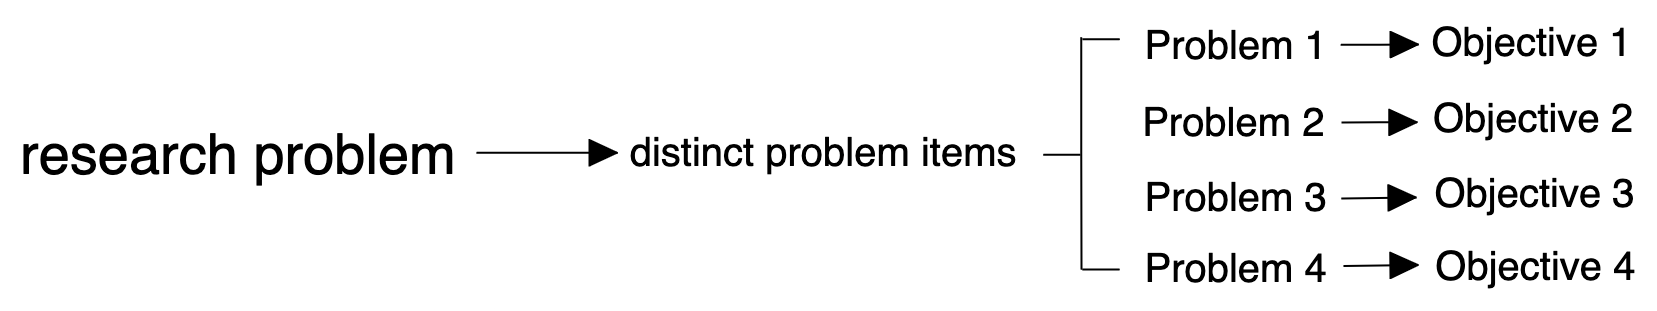
\includegraphics[width=0.75\linewidth]{assets/problem-to-objective-mapping.png}
	\caption{Inference of objectives from problems.
		%		(\citeauthor{ref}, \citeyear{ref}).
	}
	\label{fig:problemToObjectiveMapping}	
\end{figure}

\subsection{Activity 2: Define Objectives of a Solution}
\label{methodology:activity2}

\noindent
In activity 2,
research objectives are inferred from the problem definition in activity 1.
Each objective maps to a distinct item from the problem specification
(illustrated in Figure \ref{fig:problemToObjectiveMapping}),
which helps with later evaluation in activity 5.
In practice, a research objective will be a qualitative description of
how a new artifact is expected to support a solution to the problem definition.
\bigskip

\subsection{Activity 3: Design \& Development}
\label{methodology:activity3}

\noindent
In activity 3,
solutions for the previously defined objectives are designed and developed
by means of producing an artifact.
This is achieved by
determining the artifact's desired functionality and its architecture,
followed by actually creating the artifact
\autocite{designScienceResearchMethodologyForInformationSystemsResearch}.
In practice this means that:
Abstract model definitions of deployment environments, as well as
promotion processes are designed;
With the specification of the model definitions in place,
the "release promotion operator" is developed as an artifact.
\bigskip

\subsection{Activity 4: Demonstration}
\label{methodology:activity4}

\noindent
In activity 4,
the in-context use of the artifact is demonstrated.
After outlining how to use the artifact to effectively provide a solution to the problem definition,
the artifact is implemented in a proof-of-concept-level prototype.
%In practice,
%the prototype 
\bigskip

\subsection{Activity 5: Evaluation}
\label{methodology:activity5}

\noindent
In activity 5,
the implementation of the artifact,
and how well it supports a solution to the problem,
is evaluated.
This is achieved by
comparing the objectives of a solution to actual observed results
from use of the artifact in the demonstration
\autocite{designScienceResearchMethodologyForInformationSystemsResearch}.
In practice this means, that
the functionality of the artifact implemented in the prototype in activity 4,
is compared with the solution objectives from activity 2.
\bigskip

\subsection{Activity 6: Communication}
\label{methodology:activity6}

\noindent
In activity 6, as a final step,
the whole conducted research is communicated by means of
disclosing
the problem and its importance,
the artifact and its utility and novelty,
and the demonstration accompanied by the evalution results
\autocite{designScienceResearchMethodologyForInformationSystemsResearch},
within the publication of a master thesis at
the University of Applied Sciences Burgenland (FH Burgenland).
In addition, it may be communicated to relevant audiences such as practicing professionals;
as well as the CNCF.


\section{Research methods}

In the following section,
the used research methods
semi-structured interview
by
\citeauthor{glaser2010experteninterviews} (\citeyear{glaser2010experteninterviews})
and
design science research methodology for information systems
by
\citeauthor{designScienceResearchMethodologyForInformationSystemsResearch} (\citeyear{designScienceResearchMethodologyForInformationSystemsResearch})
are explained in detail.
%The procedure in the course of the research work is also described.

\subsection{Semi-structured interview}

%TODO: add more theory from \citeauthor{glaser2010experteninterviews} (\citeyear{glaser2010experteninterviews})

For \nameref{methodology:activity1},
semi-structured interviews with working professionals
are conducted.
These interviews have the primary goal of aiding with
problem identification and motivation,
because prior written scientific literature is insufficient on the topic.
For conducting the interviews,
a semi-structured interview guide (Appendix \ref{appendix:interview-guide}) is used.
For this research method,
the suggested practices and guideline from
the textbook of
\citeauthor{glaser2010experteninterviews} (\citeyear{glaser2010experteninterviews})
is used.

\subsubsection{Preparing the interviews}

As an initial step,
a semi-structured interview guide is developed.
It serves as a rough guideline for the structure of the interview process.
Additionally it encompasses the content-related interview questions,
which are specific to the given research problem.
These questions can be seen at section \ref{appendix:interview-questions} in the appendix.

The selection of the interview partners is based on the questions mentioned in
\citeauthor{glaser2010experteninterviews} (\citeyear{glaser2010experteninterviews}):

\begin{itemize}
	\item Who has the information relevant to this work?
	\item Who can describe it precisely?
	\item Who is most willing to be interviewed?
	\item Who is available?
\end{itemize}

The pool of potential interview partners is mainly oriented around
contacts from friends and acquaintances,
who are working professionally in the GitOps field.

\subsubsection{Conducting the interviews}

Appointments for the interviews are made with each interview partner in advance. 
The interviews are conducted in a web video conference.
The interviews are recorded for later evaluation.
The developed semi-structured interview guide
is used as a guideline for the interview process.
The actual structure of the interview differs for each individual interview partner.

\subsubsection{Transcription and post-processing of the interviews}

The output of the interviews are in the form of audio recordings.
These are transcribed word-for-word into a written form afterwards.
The content-related answers of the interview partners are taken into consideration
for \nameref{methodology:activity1}.

\subsection{Design science research methodology for information systems}

%TODO: present theory of this method

%Design science research methodology for information systems (DSRM)










%\section{Approach}
%Alle im durchgeführten Untersuchungen und Versuche müssen systematisch und
%nachvollziehbar sein. Daher ist die gewählte Vorgangsweise genau zu beschreiben
%und zu begründen. Es empfiehlt sich, dafür Literatur zum wissenschaftlichen Arbeiten
%heranzuziehen.
%
%\section{Research methods}
%Die eingesetzte Methoden (z.B. Online-Befragung, Inhaltsanalyse, Interviews) müssen
%ebenfalls nachvollziehbar beschrieben werden.
%Unterschiedliche Untersuchungsmethoden haben oft unterschiedliche Genauigkeit.
%Neben der Begründung und Beschreibung der Untersuchungsmethoden ist auch eine
%Begründung und Beschreibung der verwendeten Auswertungsmethoden bzw. dafür
%verwendete Software unerlässlich\footnote{Wenn der Abstand zwischen Fußnotentrennstrich und Fußnote zu groß wird, gehen Sie folgend vor:
%	Wählen Sie im Hauptmenü „Ansicht | Entwurf | Verweise | Notizen anzeigen |
%	Fußnotentrennlinie". Dann können Sie unnötige Leerzeichen entfernen.
%}.
%Wenn es ein Kapitel 3.2.1 gibt, muss es auch ein Kapitel 3.2.2 geben.

%\subsubsection{<<Überschrift 4. Ebene>>}
%4 Überschriftenebenen müssen reichen.
%
%
%\section{Displayed Text}
%Text is displayed by indenting it from the left
%margin.  Quotations are commonly displayed.  There
%are short quotations
%\begin{quote}
%	This is a short quotation.  It consists of a 
%	single paragraph of text.  See how it is formatted.
%\end{quote}
%and longer ones.
%\begin{quotation}
%	This is a longer quotation.  It consists of two
%	paragraphs of text, neither of which are
%	particularly interesting.
%	
%	This is the second paragraph of the quotation.  It
%	is just as dull as the first paragraph.
%\end{quotation}
%Another frequently-displayed structure is a list.
%The following is an example of an \emph{itemized}
%list.
%\begin{itemize}
%	\item This is the first item of an itemized list.
%	Each item in the list is marked with a ``tick''.
%	You don't have to worry about what kind of tick
%	mark is used.
%	
%	\item This is the second item of the list.  It
%	contains another list nested inside it.  The inner
%	list is an \emph{enumerated} list.
%	\begin{enumerate}
%		\item This is the first item of an enumerated 
%		list that is nested within the itemized list.
%		
%		\item This is the second item of the inner list.  
%		\LaTeX\ allows you to nest lists deeper than 
%		you really should.
%	\end{enumerate}
%	This is the rest of the second item of the outer
%	list.  It is no more interesting than any other
%	part of the item.
%	\item This is the third item of the list.
%\end{itemize}
%You can even display poetry.
%\begin{verse}
%	There is an environment 
%	for verse \\             % The \\ command separates lines
%	Whose features some poets % within a stanza.
%	will curse.   
%	
%	% One or more blank lines separate stanzas.
%	
%	For instead of making\\
%	Them do \emph{all} line breaking, \\
%	It allows them to put too many words on a line when they'd rather be 
%	forced to be terse.
%\end{verse}
%
%Mathematical formulas may also be displayed.  A
%displayed formula 
%is 
%one-line long; multiline
%formulas require special formatting instructions.
%\[  \Gamma \times  \psi = x'' + y^{2} + z_{i}^{n}\]
%Don't start a paragraph with a displayed equation,
%nor make one a paragraph by itself.
